 \section{Application to air pollution forecasting}
      
   \subsection{Description of the data}

      \subsubsection{Exploratory data analysis}
      
         \begin{table}[H]
            \centering
            \begin{tabularx}{\textwidth}{|l|l|X|l|}
            \hline
            \text{Variable} & \text{Name} & \text{Description} & \text{Unit} \\
            \hline
            \(\text{NO}_{2}\) & Nitrogen dioxide & A harmful gas from vehicles and industry. & \(\mu\text{g}/\text{m}^{3}\) \\
            \(\text{PM}_{10}\) & Particulate matter 10 & Small inhalable dust particles. & \(\mu\text{g}/\text{m}^{3}\) \\
            \(\text{SO}_{2}\) & Sulphur dioxide & Mainly from burning fossil fuels. & \(\mu\text{g}/\text{m}^{3}\) \\
            Speed & Wind speed & How fast the wind is moving. & m/s \\
            \hline
            \end{tabularx}
            \caption{\textit{Description of variables of the air pollution dataset.}}
            \label{tab:variable_description}
         \end{table}

         \begin{figure}[H]
            \centering
            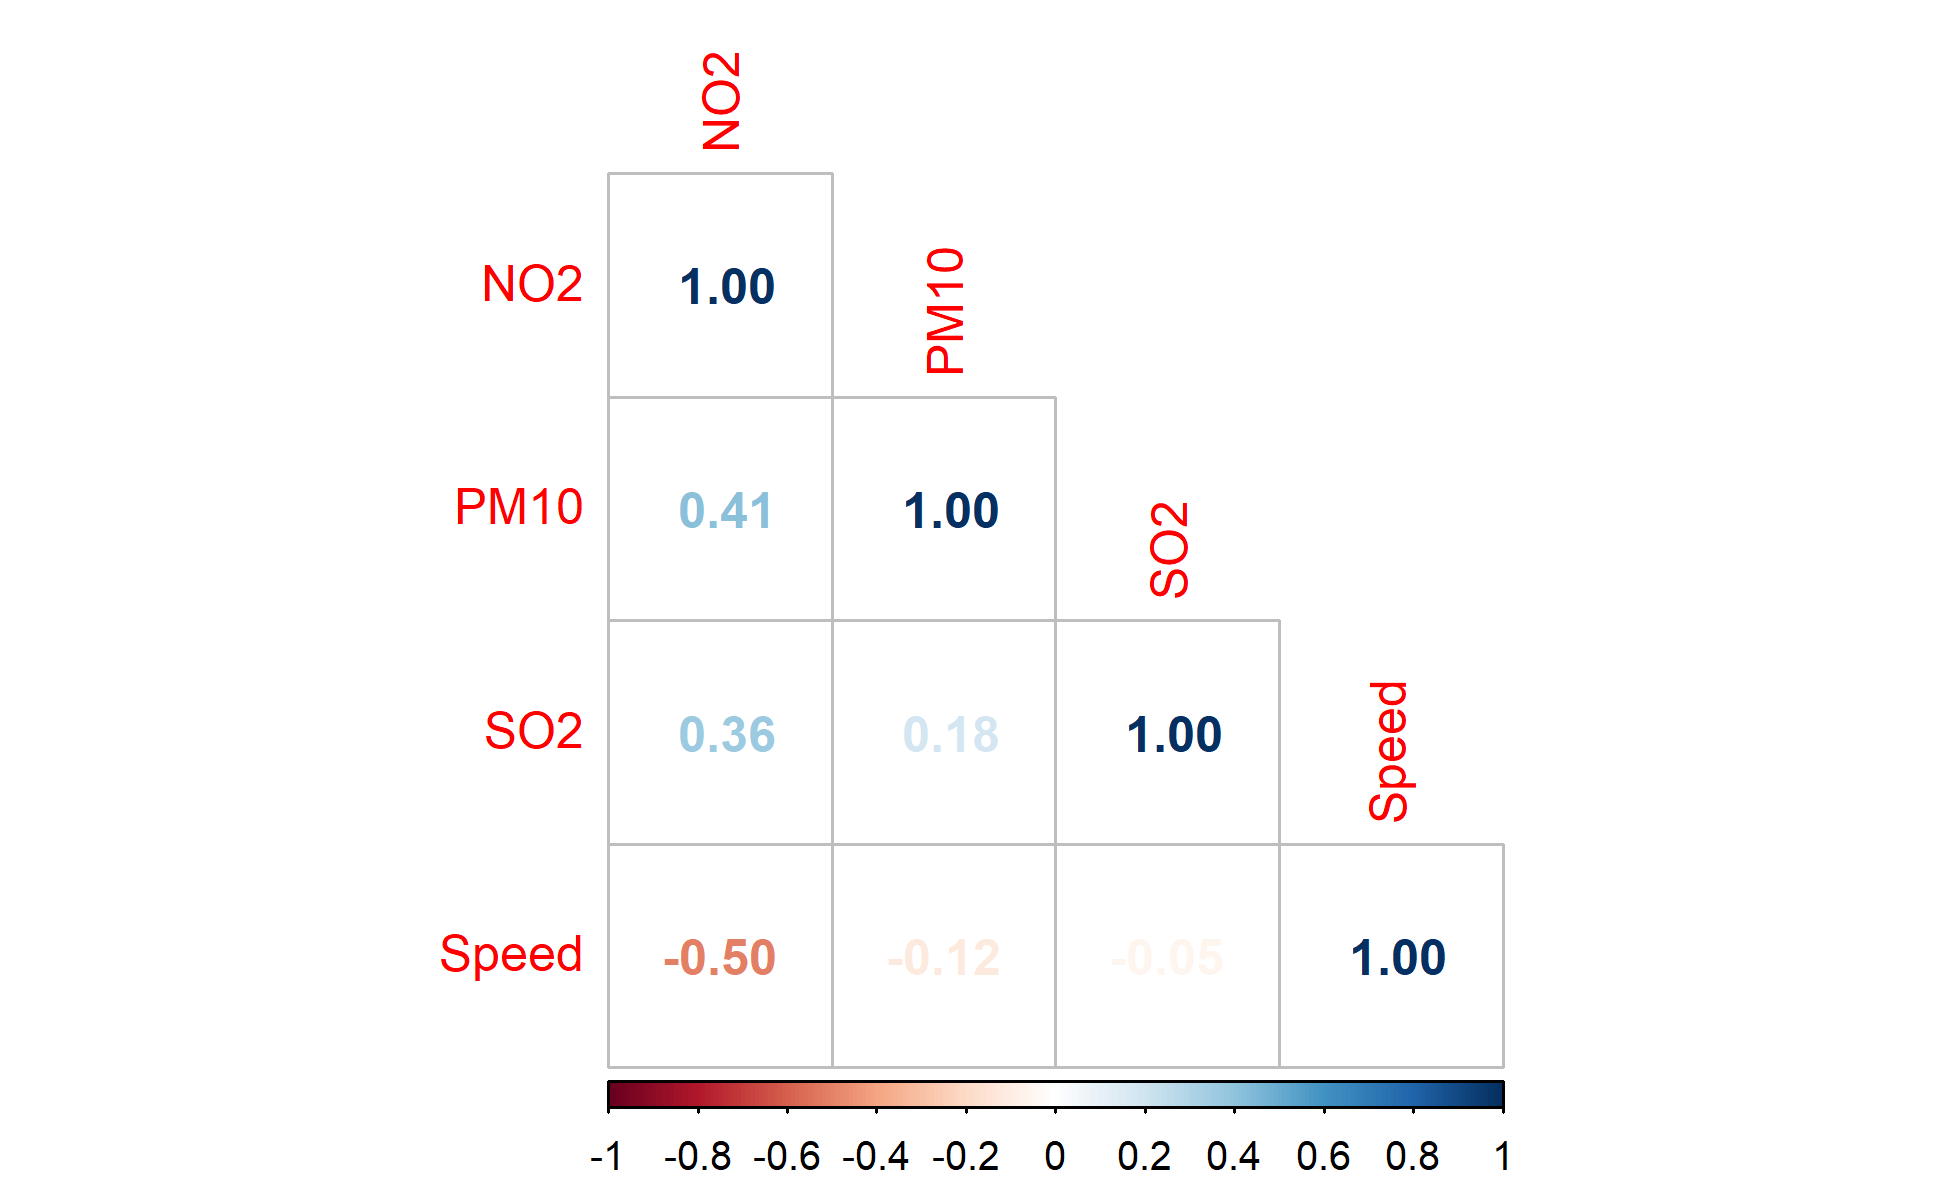
\includegraphics[width=0.48\linewidth]{../images/corrplot.png}
            \caption{\textit{Correlation plot of the air pollution dataset.}}
         \end{figure}

         Our response variable $\text{NO}_{2}$ appears to be moderately positively correlated with $\text{PM}_{10}$ and $\text{SO}_{2}$, and moderately negatively correlated with Speed. These are not ideal explanatory variables since we typically would like them to be strongly correlated with the response variable. The explanatory variables are weekly correlated with one another, whether it be positive or negative correlation. This is ideal since some models do not work well with correlated explanatory variables, often leading to unstable point estimates and inflated standard errors.

         \begin{figure}[H]
            \centering
            \begin{subfigure}{0.48\linewidth}
               \centering
               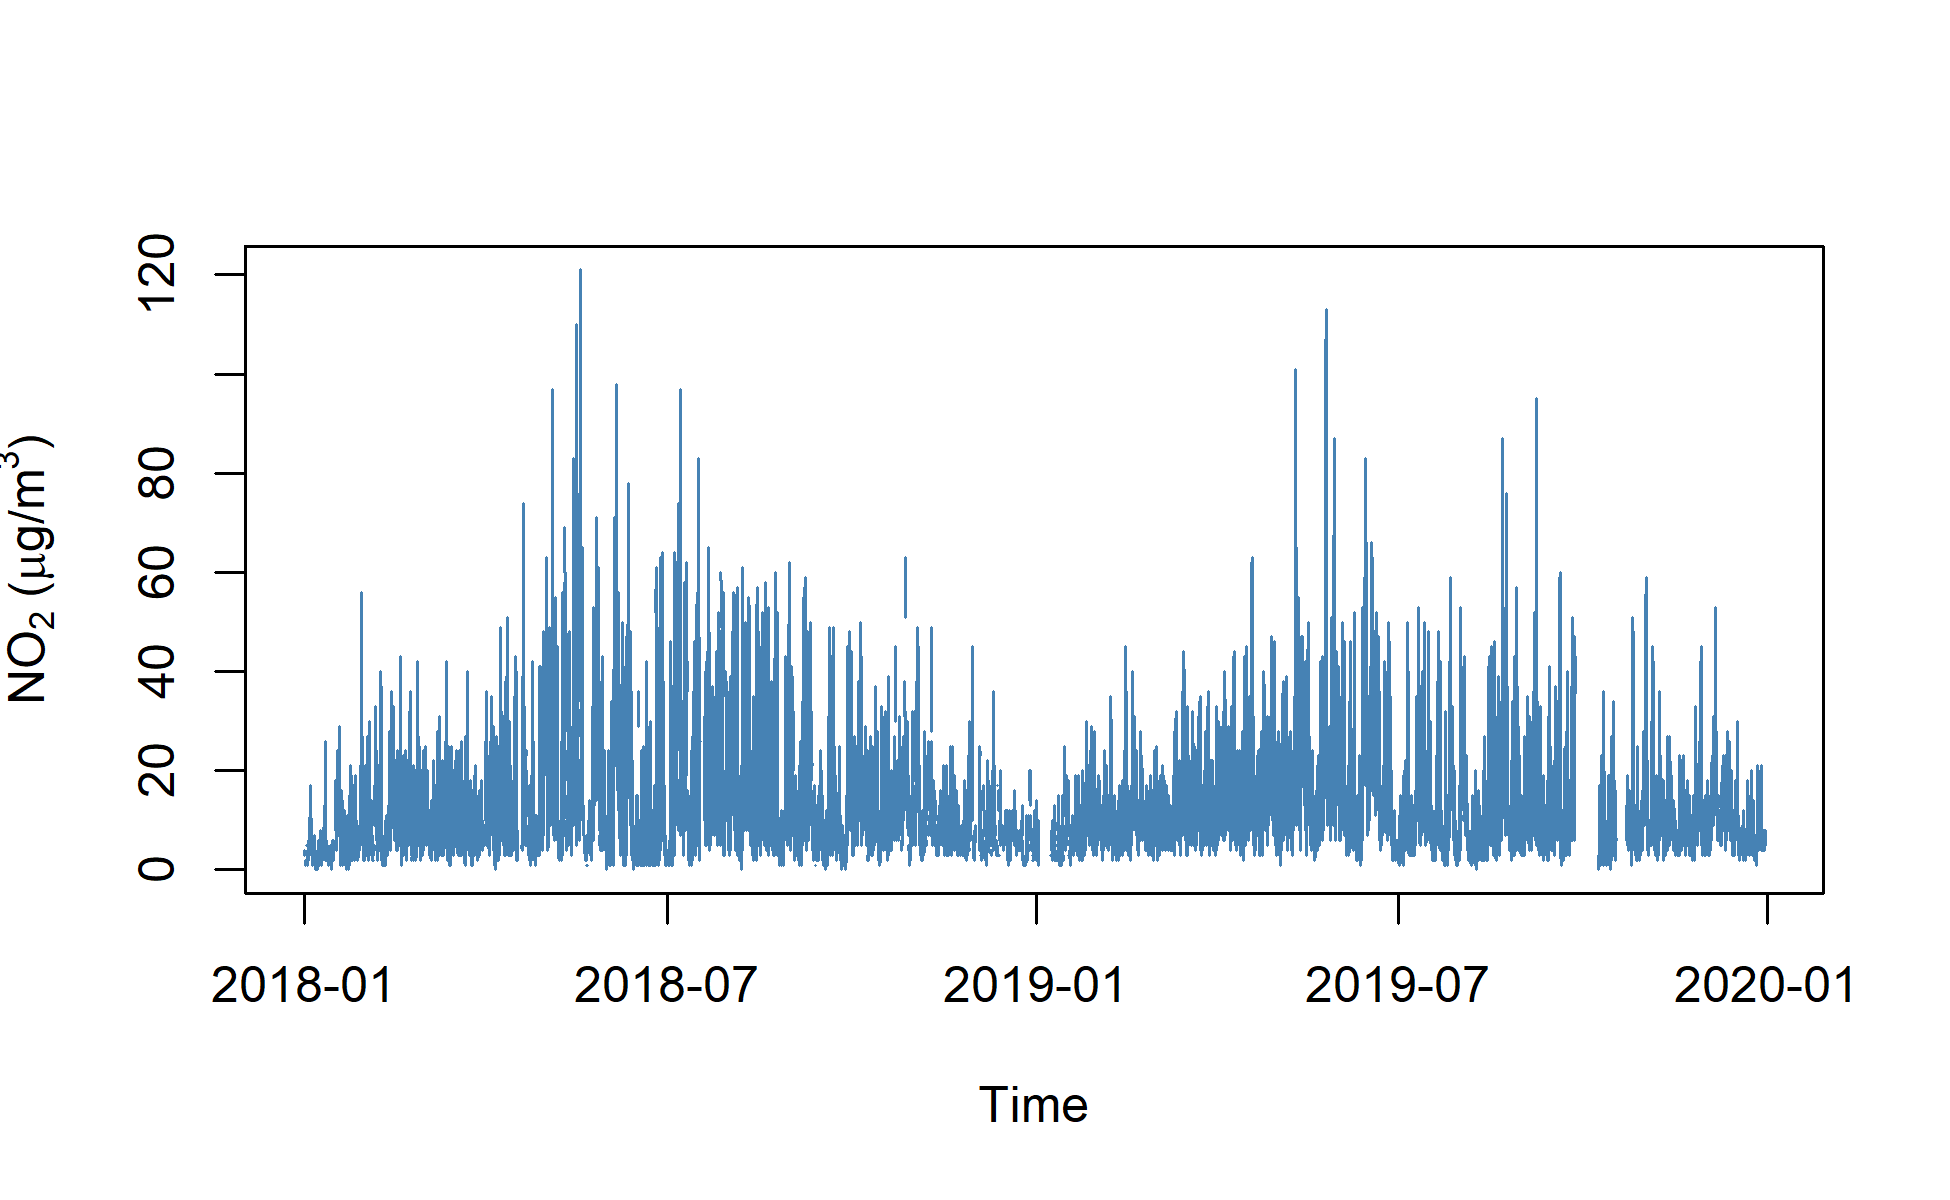
\includegraphics[width=\linewidth]{../images/extracted_no2.png}
            \caption{Nitrogen dioxide}
            \end{subfigure}
            \hfill
            \begin{subfigure}{0.48\linewidth}
               \centering
               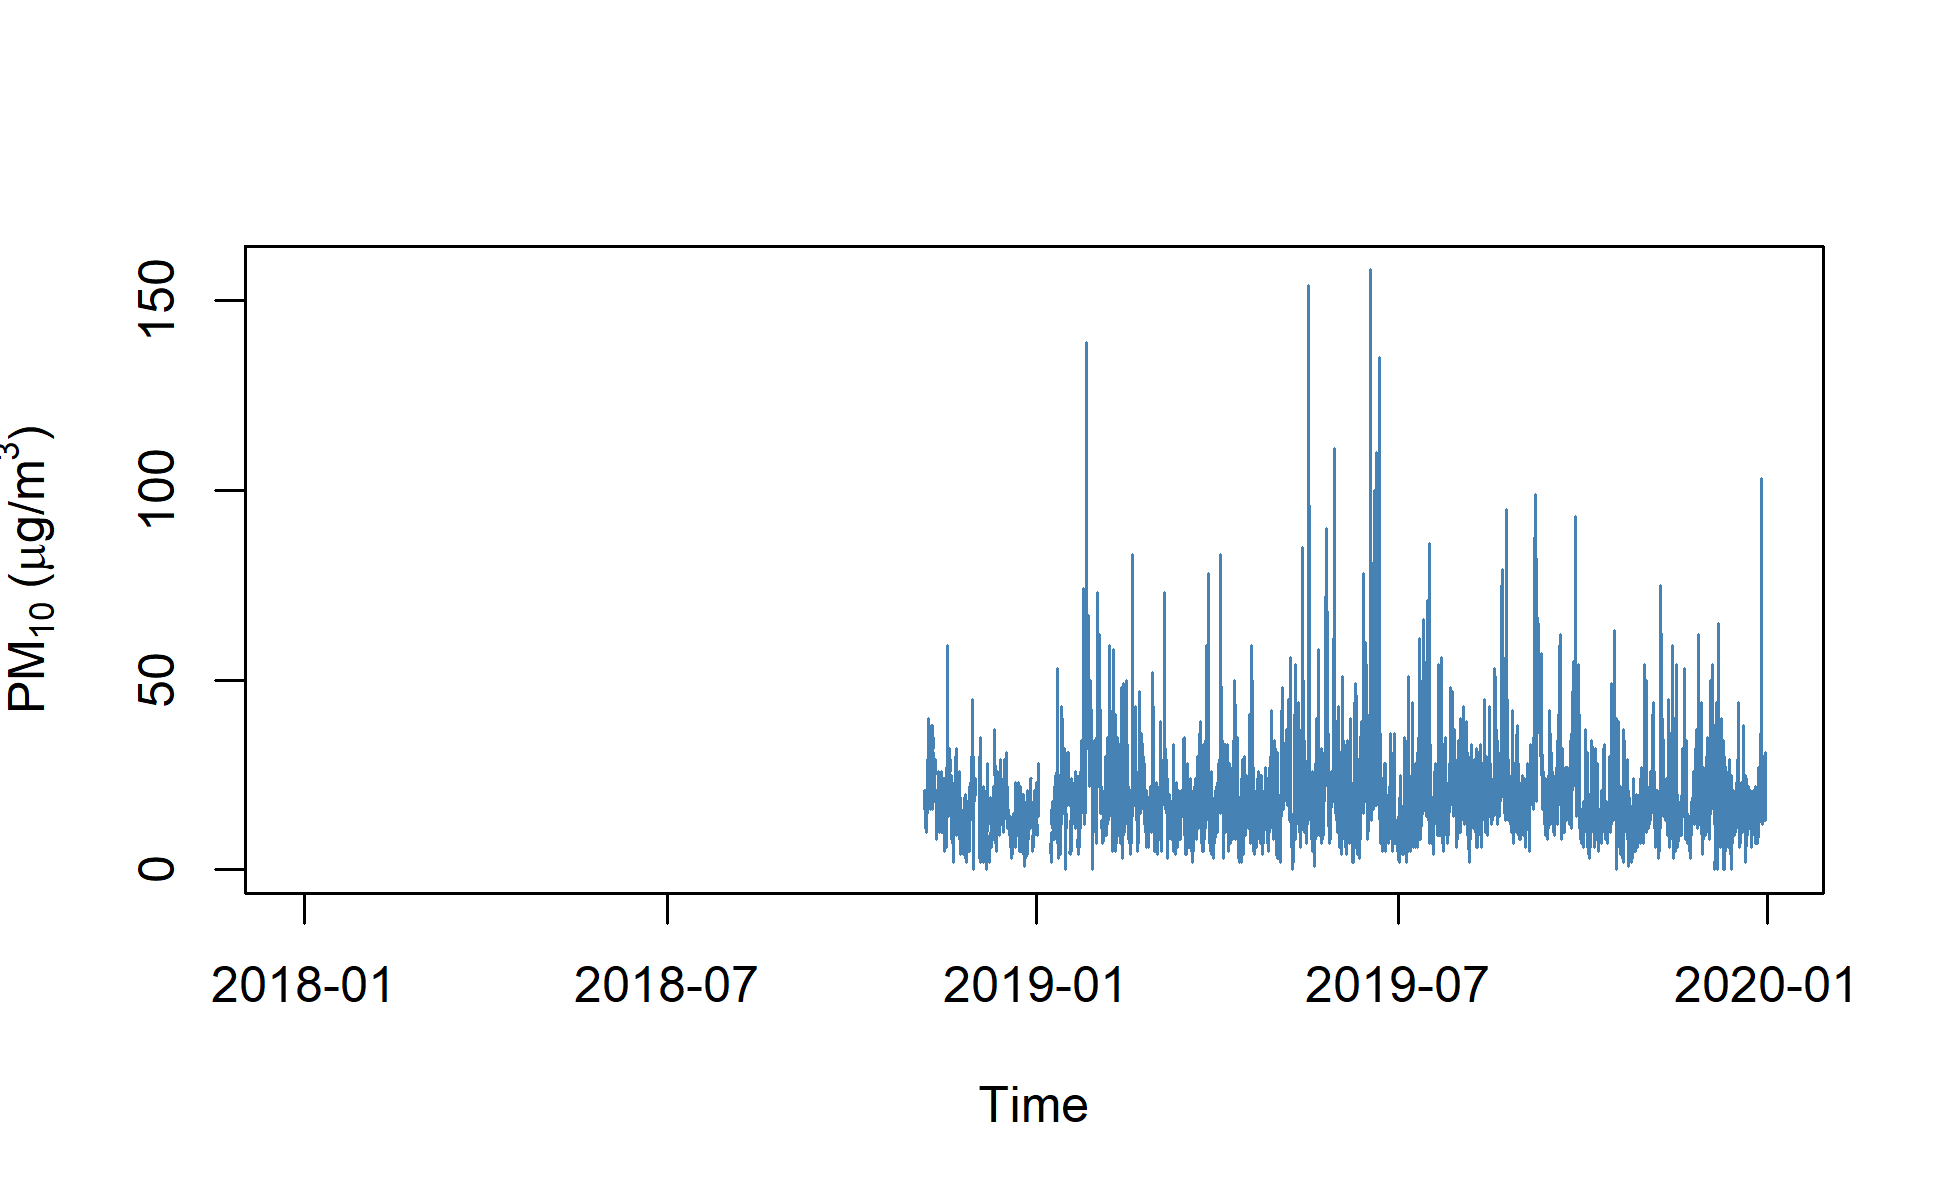
\includegraphics[width=\linewidth]{../images/extracted_pm10.png}
               \caption{Particulate matter 10}
            \end{subfigure}
            
            \vspace{0.5em}

            \begin{subfigure}{0.48\linewidth}
               \centering
               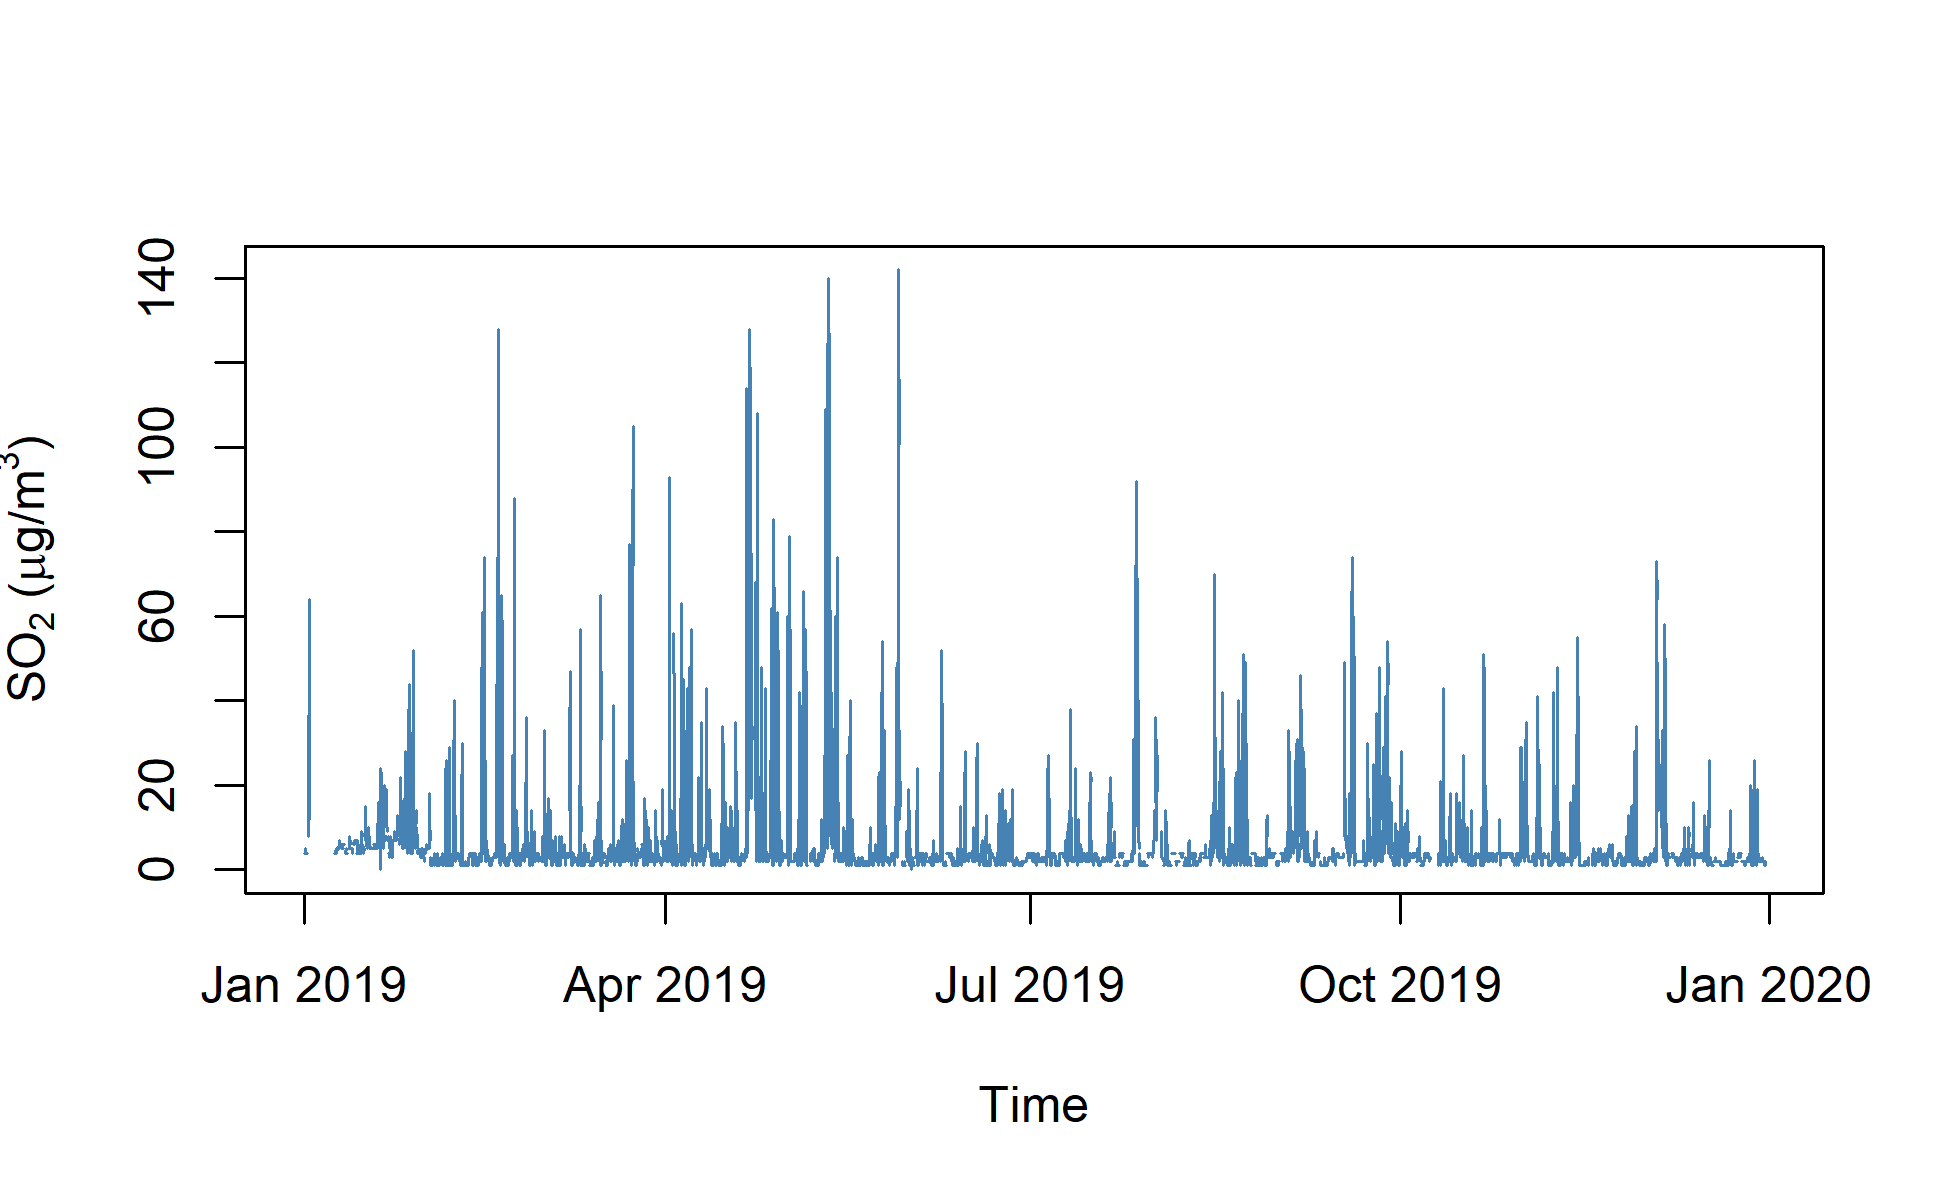
\includegraphics[width=\linewidth]{../images/extracted_so2.png}
            \caption{Sulphur dioxide}
            \end{subfigure}
            \hfill
            \begin{subfigure}{0.48\linewidth}
               \centering
               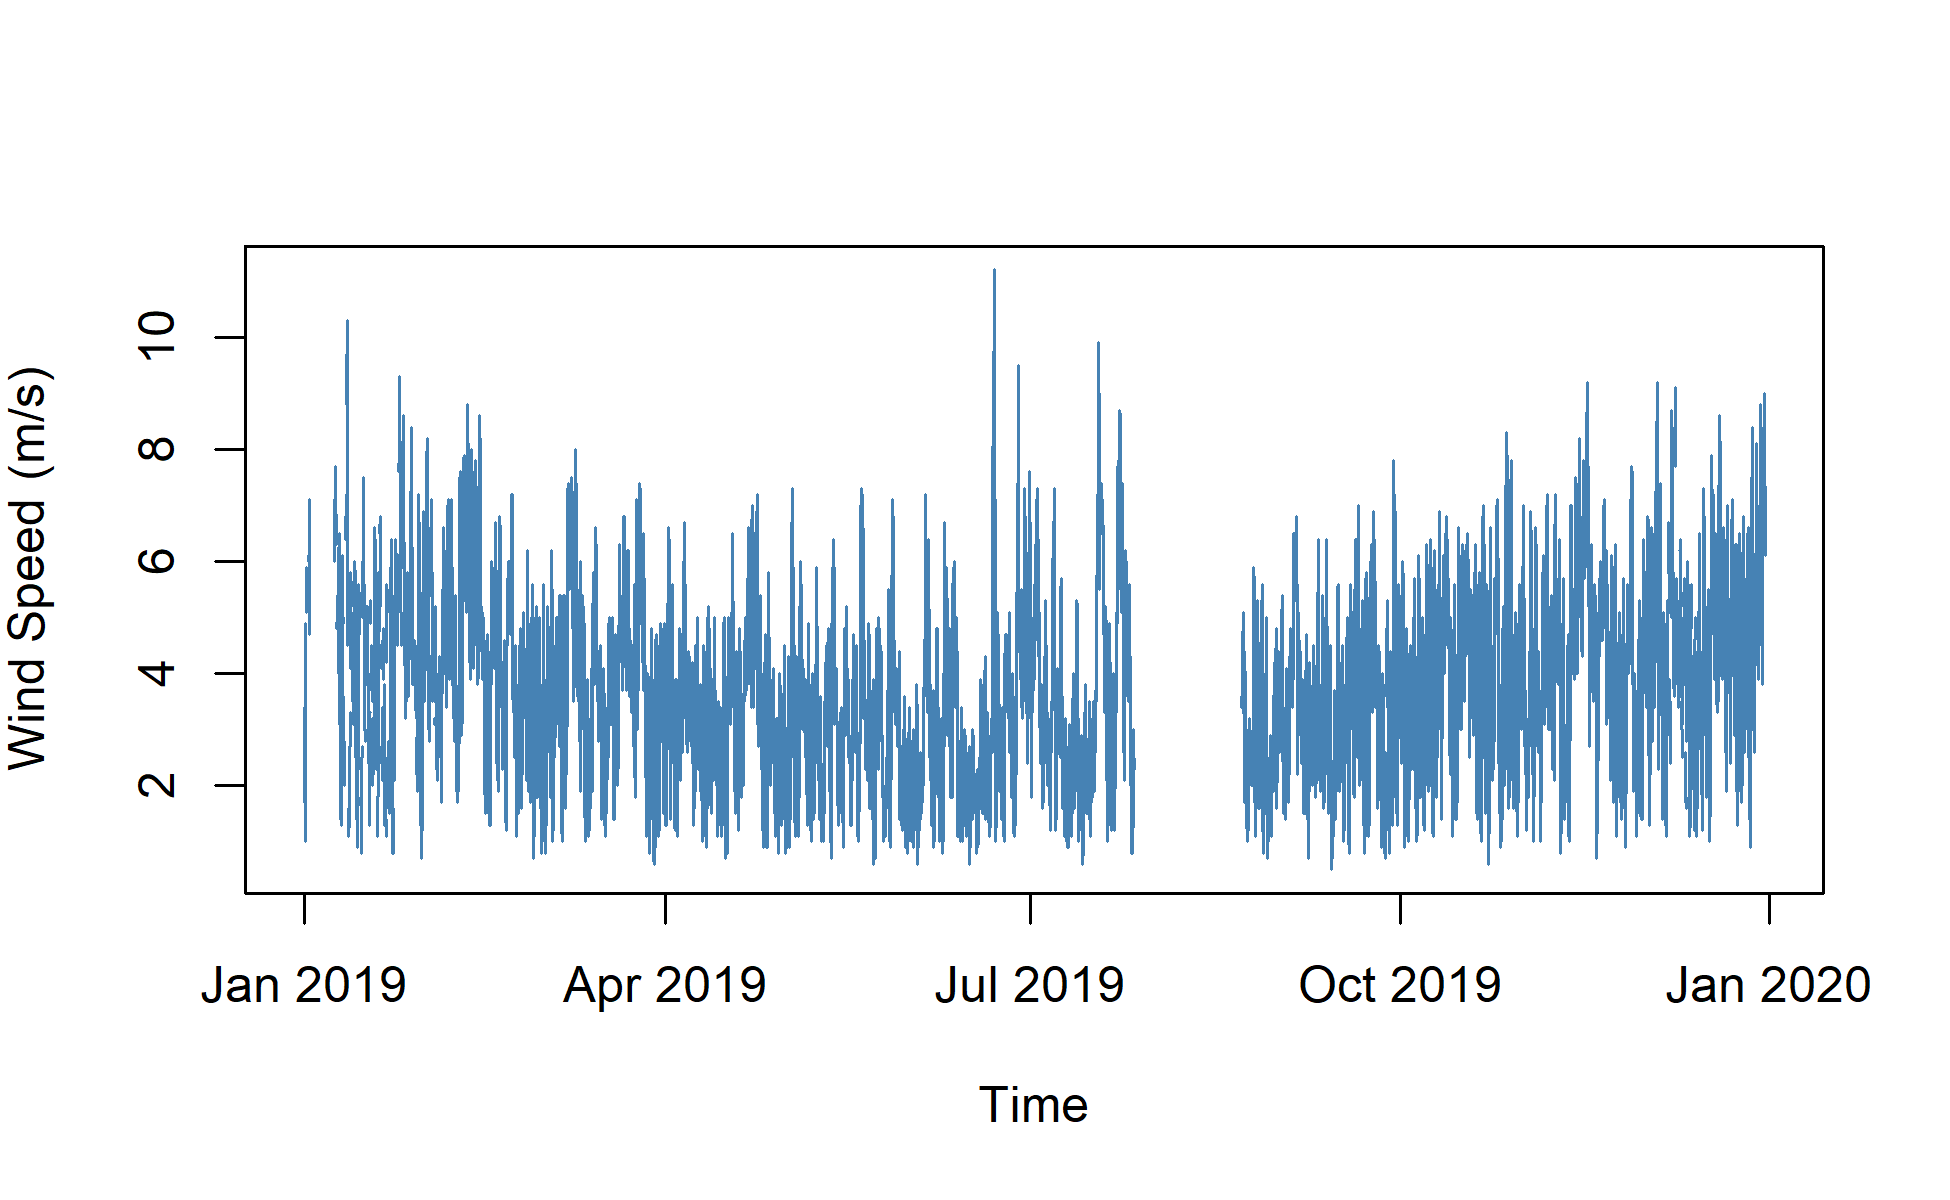
\includegraphics[width=\linewidth]{../images/extracted_speed.png}
               \caption{Wind speed}
            \end{subfigure}

            \caption{\textit{Time-series plots of nitrogen dioxide and meteorological processes from 01/01/2018 to 31/12/2019 measured hourly. Similar cyclic patterns can be observed in the meteorological processes, and a weaker seasonality component can be noted in the yearly nitrogen dioxide processes.}}
         \end{figure}

      \subsubsection{Data pre-processing}

         The response variable time-series $x_{t}$ is not stationary because the mean and variance are changing with time. To achieve stationarity there is a need for de-trending and a variance stabilizing transformation. In order to stabilize the variance we use Box-Cox transformations in the training set, $y_{t} = (x_{t}^{\lambda} - 1) / \lambda$. The Box-Cox transformations allow us to experiment with a wide variety of $\lambda$ values. A good value of $\lambda$ is one the makes the variation in the data constant through time \cite{Watson2025}. The \texttt{R} package \texttt{forecast} was used to perform the Box-Cox transformation which yielded an optimal value of $\hat{\lambda} \approx 0$, suggesting a logarithmic transformation. Then, conducting first-order differencing at lag one to remove the trend $z_{t} = y_{t} - y_{t-1} \, \text{for} \, t \in \{2, \, 3, \, \ldots, \, p\}$. The time series $z_{t}$ is now stationary. Thus, we only need to account for the mean and variance in our models.

         \begin{figure}[H]
            \centering
            \begin{subfigure}{0.48\linewidth}
               \centering
               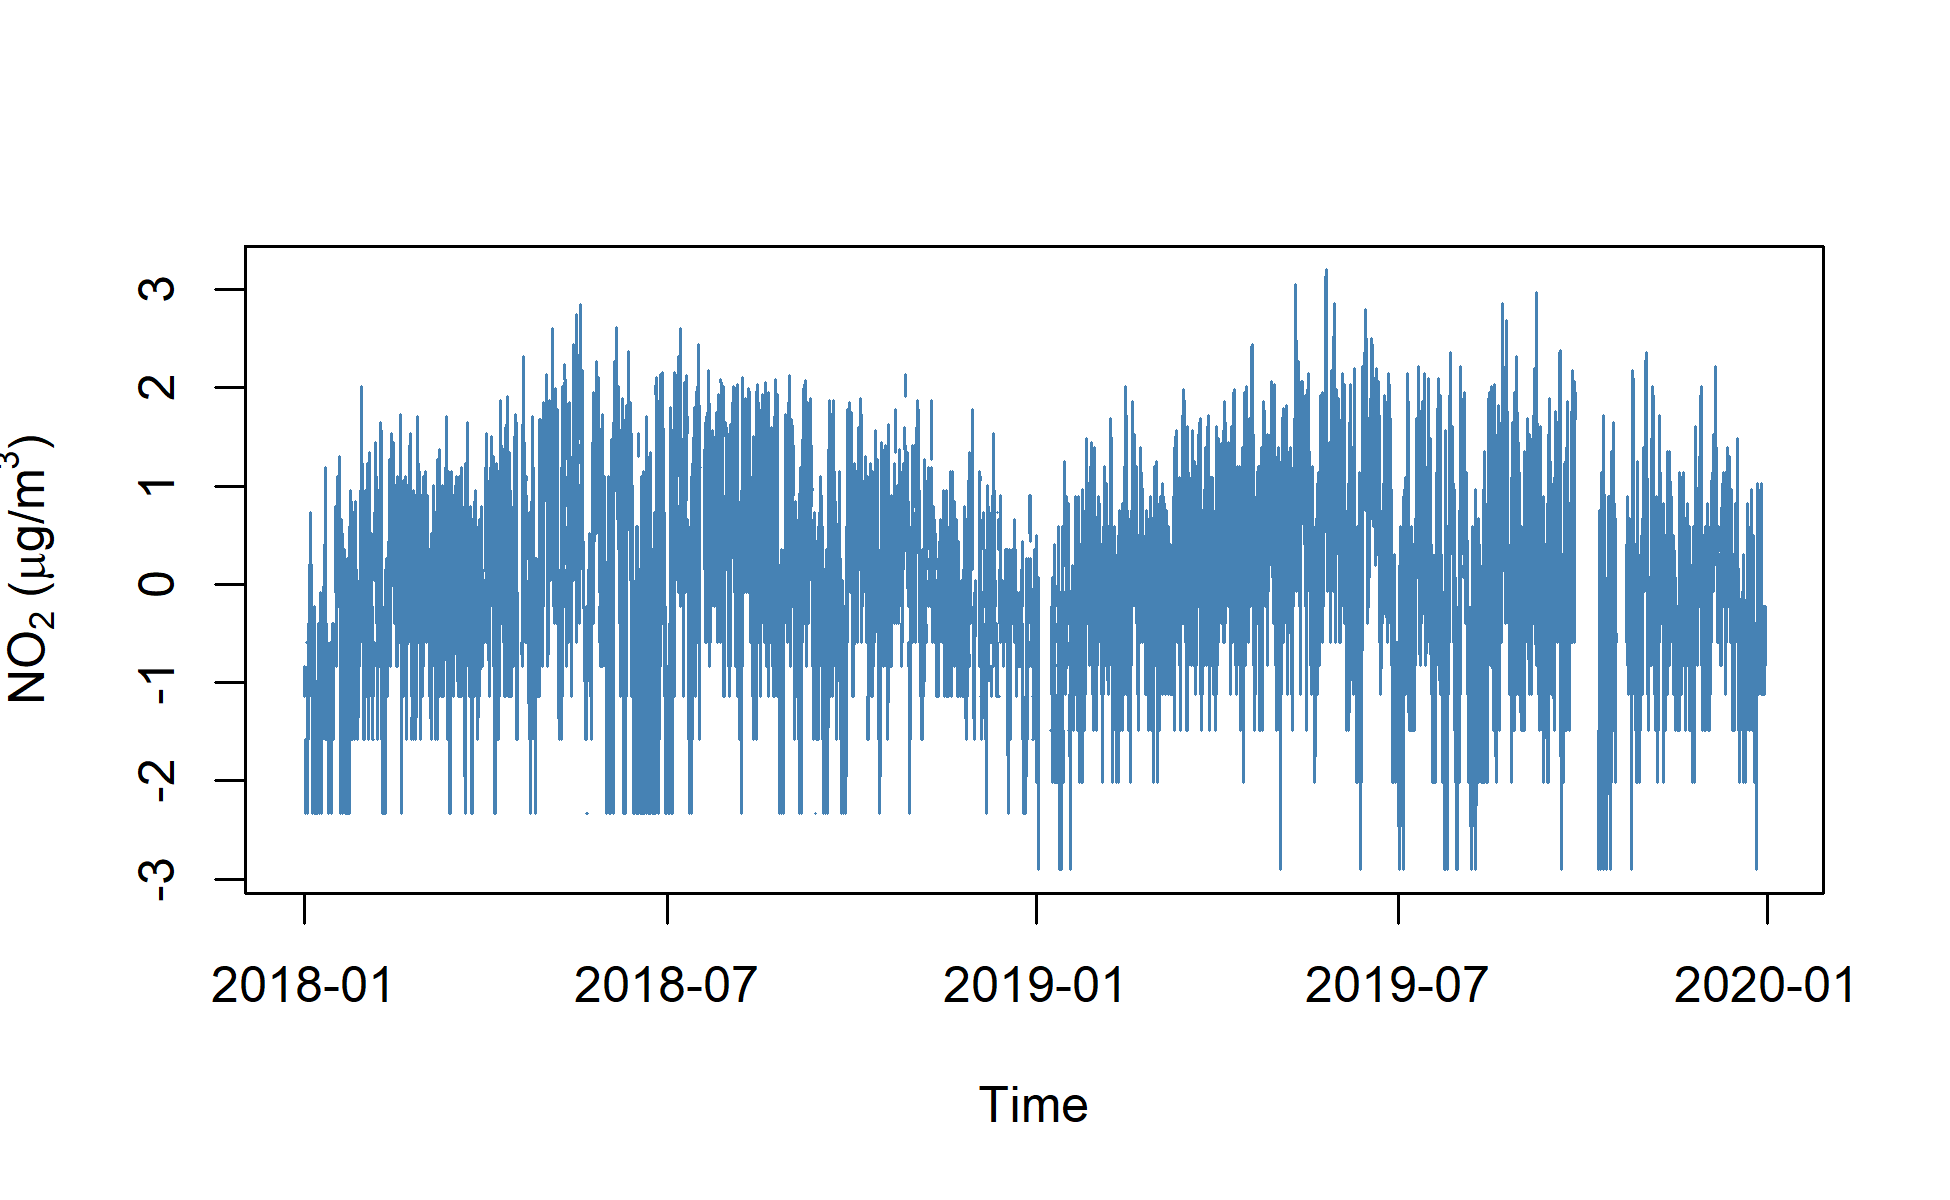
\includegraphics[width=\linewidth]{../images/transformed_no2.png}
            \caption{Nitrogen dioxide}
            \end{subfigure}
            \hfill
            \begin{subfigure}{0.48\linewidth}
               \centering
               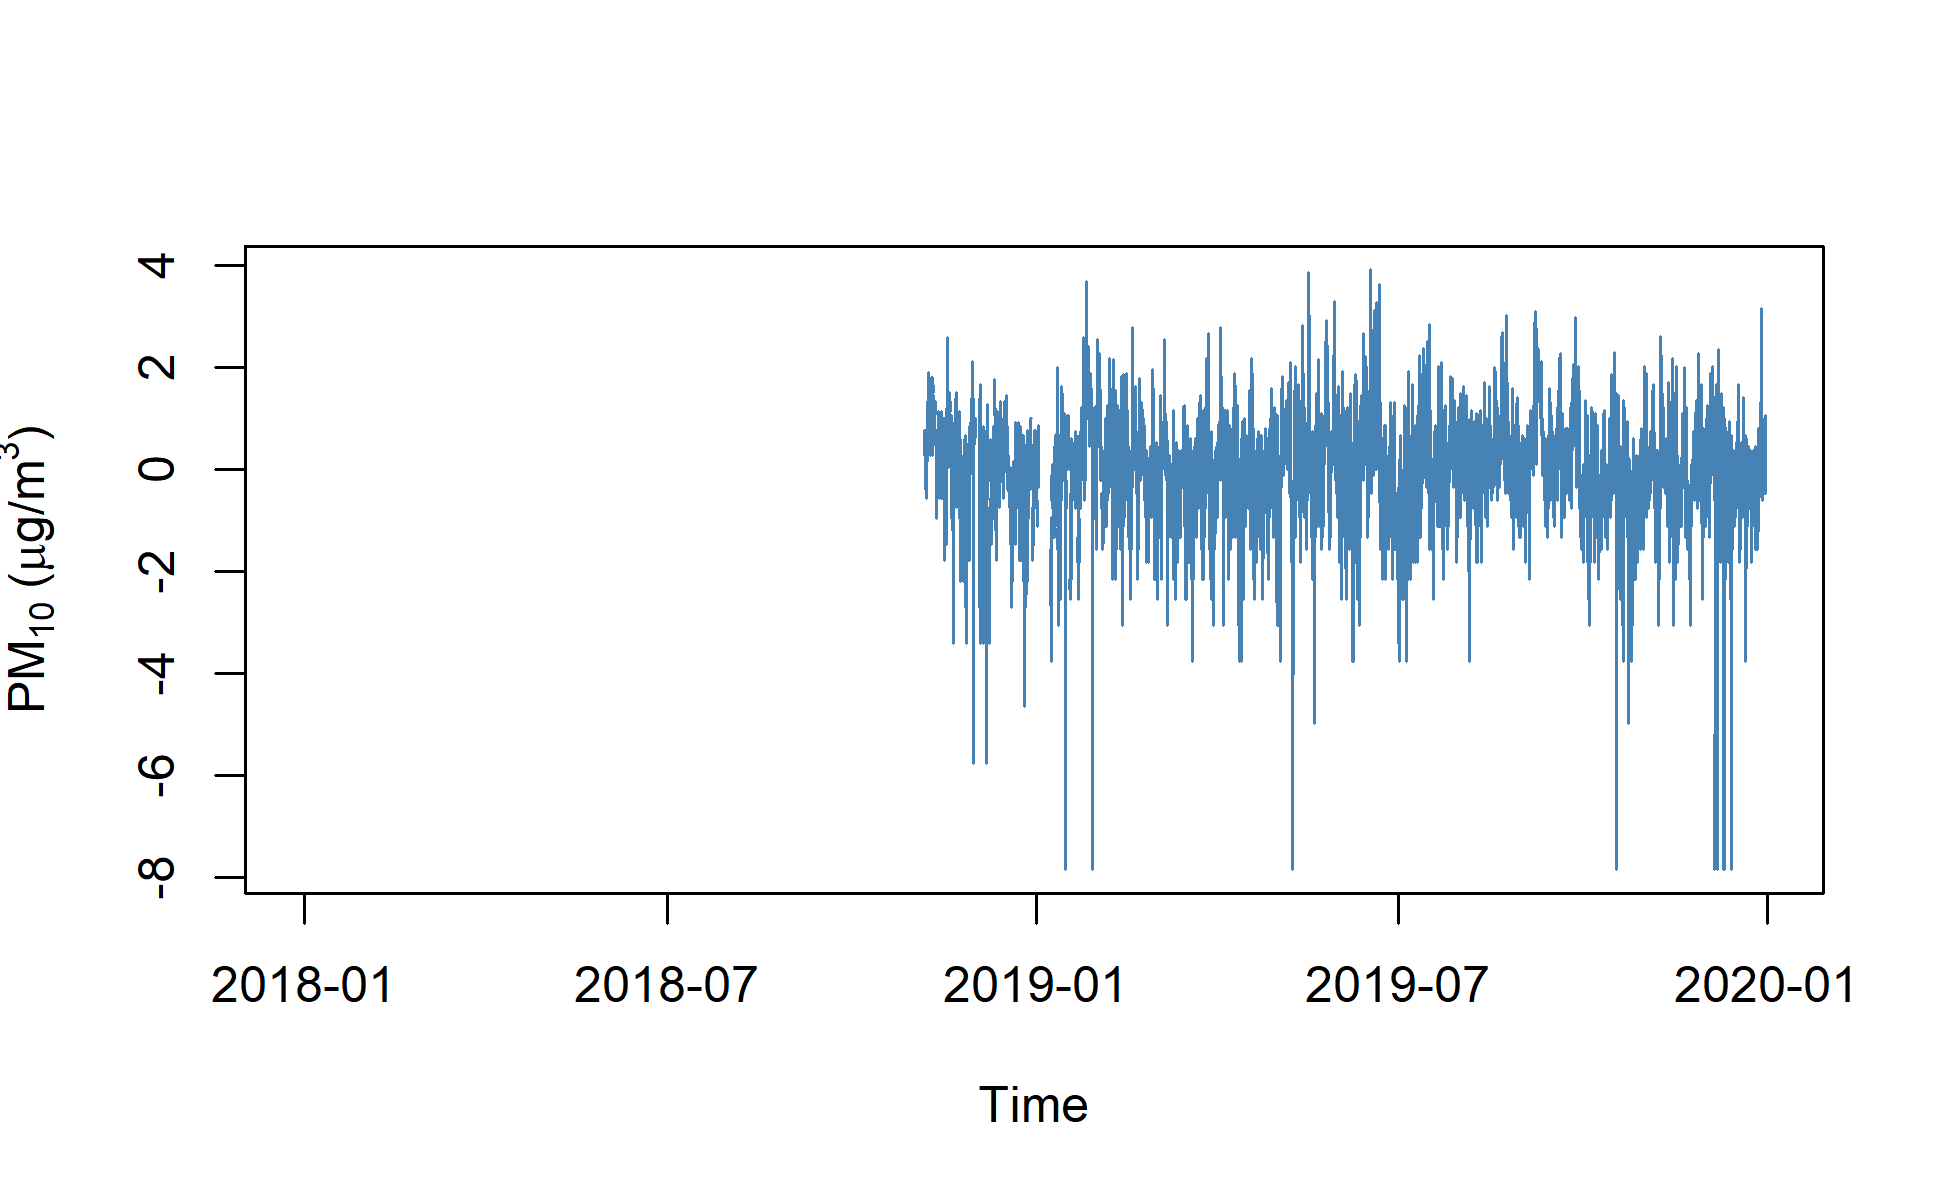
\includegraphics[width=\linewidth]{../images/transformed_pm10.png}
               \caption{Particulate matter 10}
            \end{subfigure}
            
            \vspace{0.5em}

            \begin{subfigure}{0.48\linewidth}
               \centering
               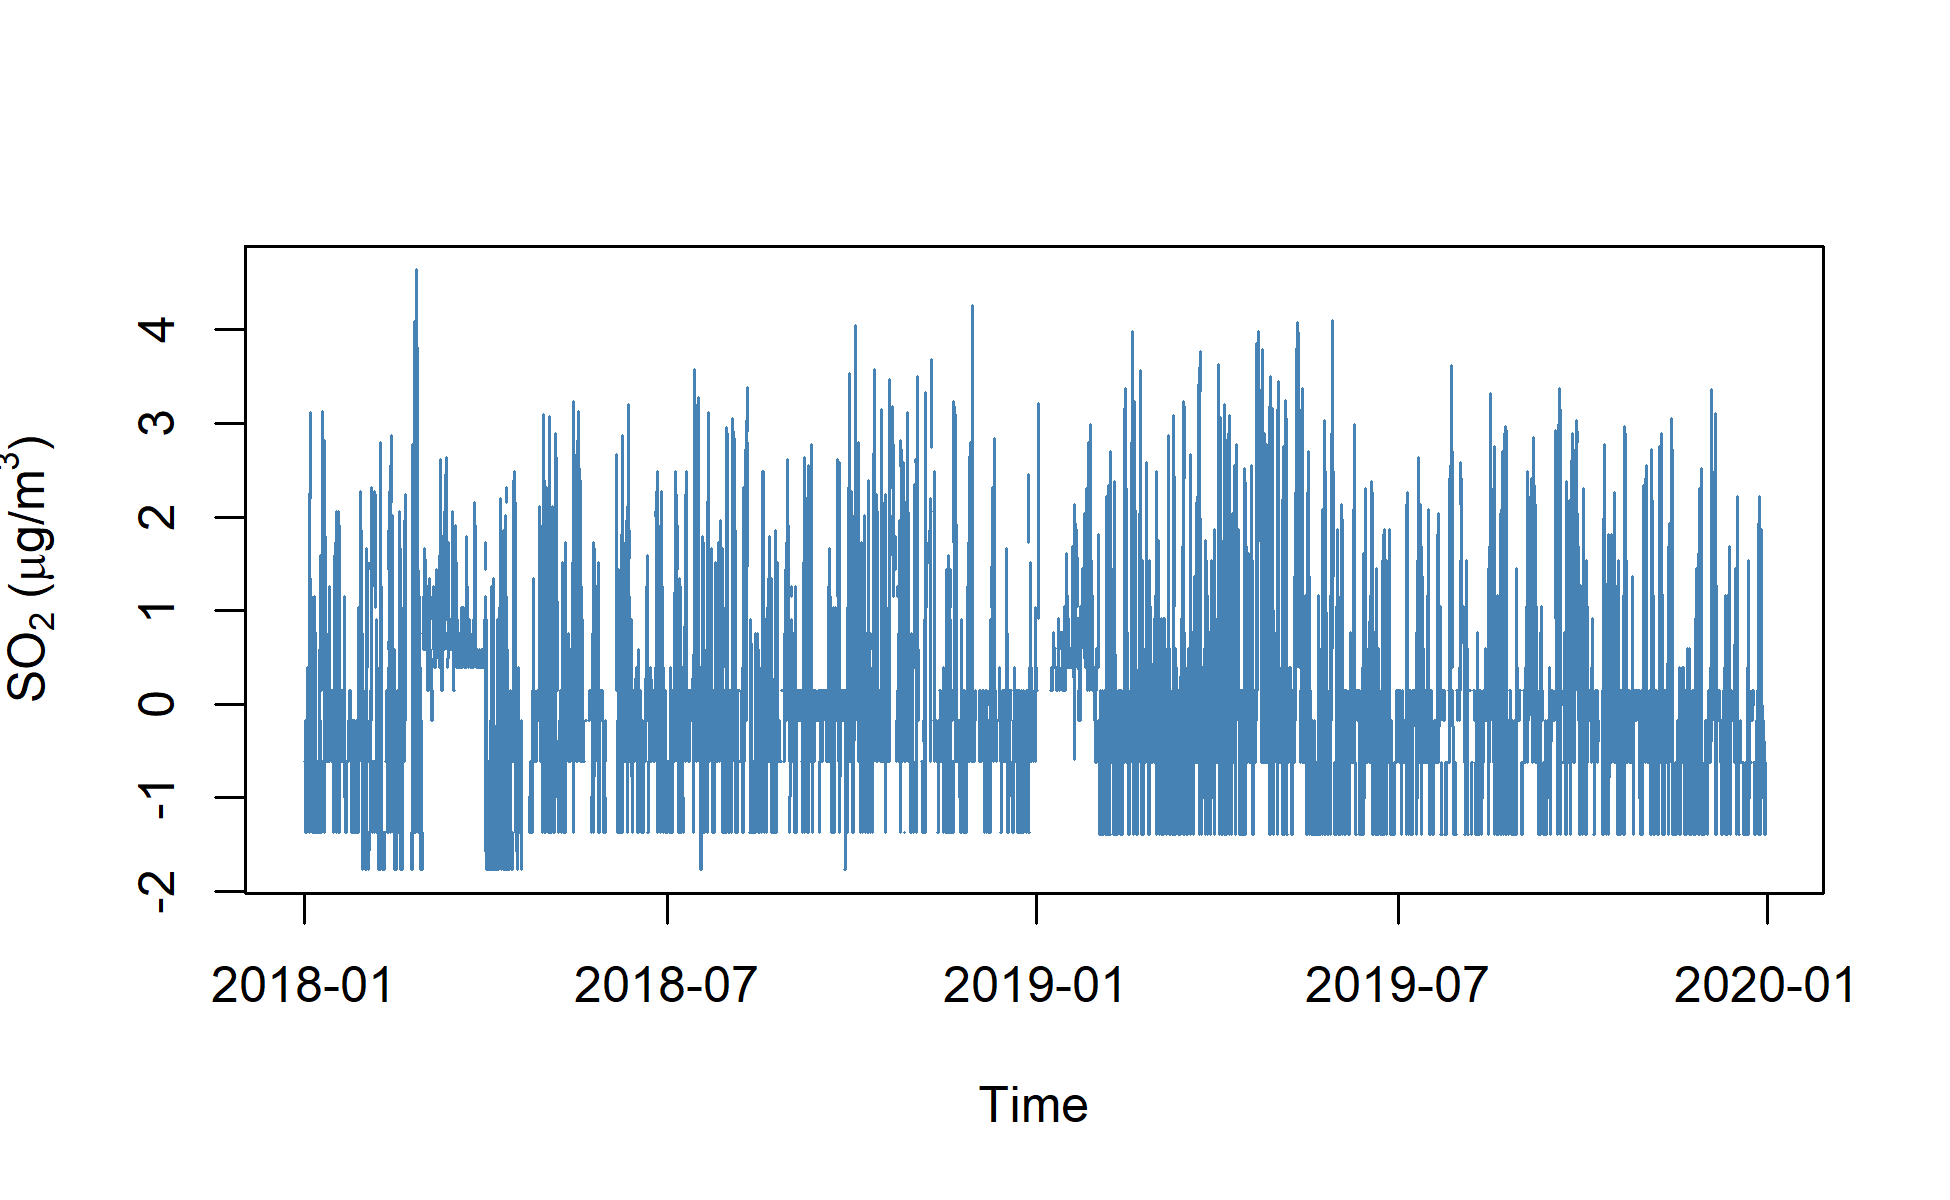
\includegraphics[width=\linewidth]{../images/transformed_so2.png}
            \caption{Sulphur dioxide}
            \end{subfigure}
            \hfill
            \begin{subfigure}{0.48\linewidth}
               \centering
               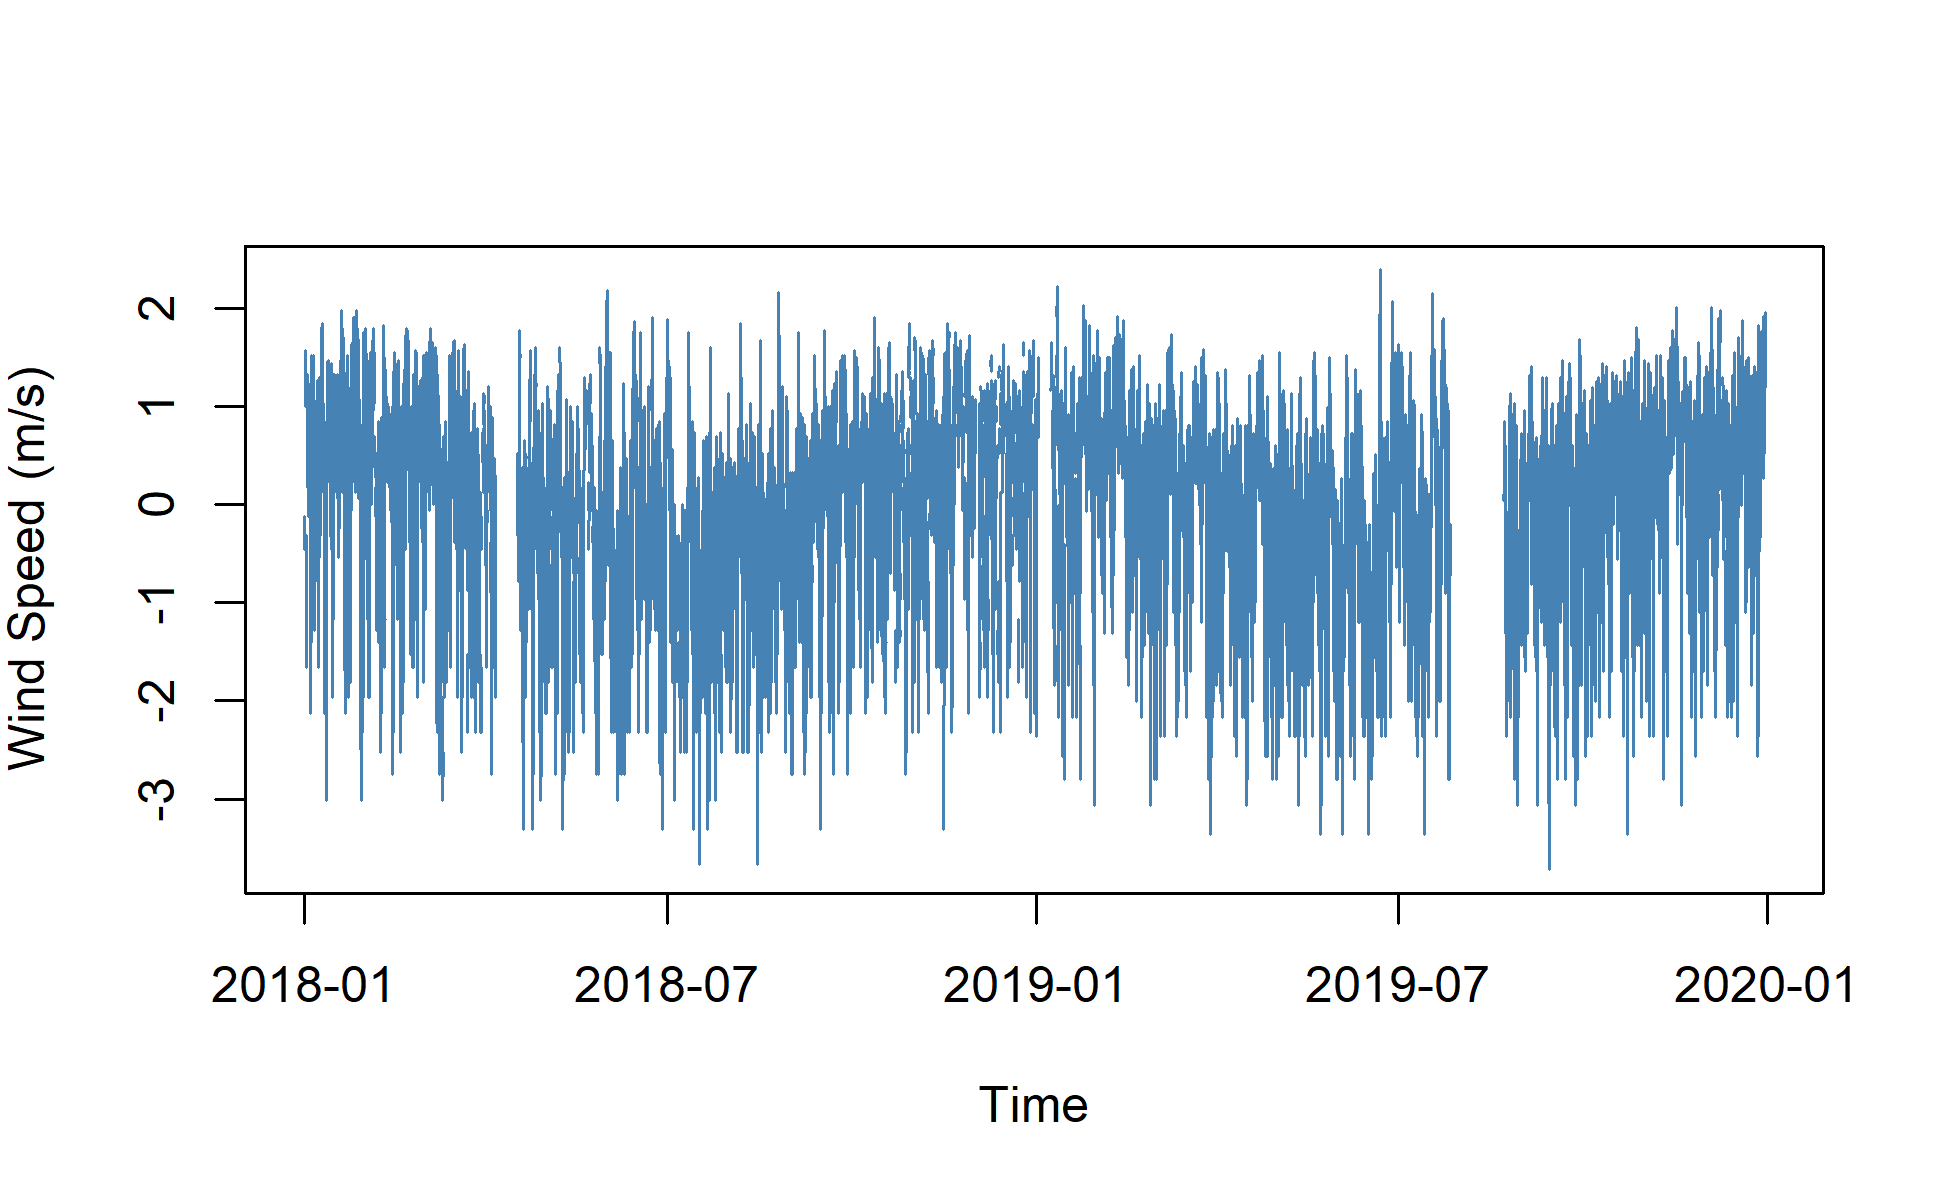
\includegraphics[width=\linewidth]{../images/transformed_speed.png}
               \caption{Wind speed}
            \end{subfigure}

            \caption{\textit{Post-processed daily curves of the nitrogen dioxide and meteorological data, both standardized by their overall mean and standard deviation.}}
         \end{figure}
   
   \subsection{Results}

      \begin{table}[H]
         \centering
         \begin{tabular}{lcccccc}
         \hline
         \multirow{2}{*}{Model} & \multicolumn{3}{c}{RMSE} & \multicolumn{3}{c}{MAE} \\
         \cline{2-7}
         & \multicolumn{3}{c}{Forecasts} & \multicolumn{3}{c}{Forecasts} \\
         & \multicolumn{3}{c}{($h$ day time horizon)} & \multicolumn{3}{c}{($h$ day time horizon)} \\
         & 24 & 168 & 744 & 24 & 168 & 744 \\
         \hline
         Average & {7.731} & \textbf{\textcolor{red}{5.397}} & {7.439} & \textbf{\textcolor{red}{6.042}} & \textbf{\textcolor{red}{4.254}} & {5.385} \\
         Naive & {10.553} & {7.864} & {10.040} & {7.708} & {6.071} & {7.308} \\
         Drift & {10.606} & {8.128} & {11.358} & {7.764} & {6.391} & {8.809} \\
         AR(1) & {8.662} & {5.912} & {8.044} & {6.029} & {4.422} & {5.616} \\
         GP-0-WN & {13.756} & {11.141} & {13.169} & {11.719} & {9.786} & {11.081} \\
         GP-0-SE & {~} & {~} & {~} & {~} & {~} & {~} \\
         GP-MLR-WN & \textbf{\textcolor{red}{7.692}} & {6.134} & \textbf{\textcolor{red}{7.225}} & {6.119} & {4.490} & \textbf{\textcolor{red}{5.136}} \\
         GP-MLR-SE & {~} & {~} & {~} & {~} & {~} & {~} \\
         \hline
         \end{tabular}
         \caption{\textit{RMSE and MAE of forecasting models across horizons.}}
      \end{table}
